% =====================================================================
%  PC-RF poster for AIAS+ 2026, A0 portrait (33.1 in x 46.8 in), XeLaTeX.
%
%  FORMAT: the AIAS+ rule is A0 portrait, 33.1 in x 46.8 in, printed and brought
%  by the presenter. The typography follows the Spatial Atlas poster (Berkeley RDI
%  Agentic AI Summit, Aug 2026) with its NVIDIA-derived green palette removed: EB
%  Garamond with Fira Mono, hairline separation, numbered sections with bold run-in
%  headers, and takeaway boxes. Two text columns sit above a full-width Resources band. The palette is the validated pair used in the
%  talk charts: blue for PC-RF, orange for RF-base.
%
%  EVIDENCE BOUNDARY: every number comes from the project's numbers ledger or from
%  the paper, and each one names its source file.
% =====================================================================
\documentclass{beamer}

% A0 portrait = 33.1 in x 46.8 in = 84.074 cm x 118.872 cm (2383.2 x 3369.6 pt).
\usepackage[orientation=portrait,size=custom,width=84.074,height=118.872,scale=1.0]{beamerposter}

\usepackage[utf8]{inputenc}
\usepackage[T1]{fontenc}
\usepackage[lining]{ebgaramond}
\usepackage{FiraMono}
\renewcommand*\sfdefault{\rmdefault}
\usepackage{amsmath,amssymb}
\usepackage{booktabs}
\usepackage{colortbl}
\usepackage{tabularx}
\usepackage{graphicx}
\usepackage{tcolorbox}
\tcbuselibrary{skins}
\usepackage{qrcode}
\usepackage{tikz}

\usetheme{default}
\setbeamertemplate{navigation symbols}{}
\hypersetup{colorlinks=false,pdfborder={0 0 0}}
\graphicspath{{figures/}{assets/}}

% ---------------------------------------------------------------------
%  PALETTE. Blue marks PC-RF and all rules and graphics. A darker blue is
%  reserved for text on white. Orange marks RF-base, the unconstrained model.
% ---------------------------------------------------------------------
\definecolor{pcblue}{HTML}{2A78D6}      % rules, graphics, accent bars
\definecolor{pcbluedark}{HTML}{1B5CA8}  % blue TEXT on white (contrast-safe)
\definecolor{pcwash}{HTML}{EAF2FC}      % light blue fill
\definecolor{pcorange}{HTML}{EB6834}    % RF-base
\definecolor{ncink}{HTML}{161616}
\definecolor{ncinktwo}{HTML}{161616}
\definecolor{ncmuted}{HTML}{161616}
\definecolor{ncline}{HTML}{E4E4E1}
\definecolor{nclinetwo}{HTML}{CCCCCC}
\definecolor{ncbgtwo}{HTML}{F5F5F3}
\definecolor{pending}{HTML}{C01C1C}

\setbeamercolor{background canvas}{bg=white}
\setbeamercolor{normal text}{fg=ncinktwo}
\usebeamercolor[fg]{normal text}
\setbeamertemplate{blocks}[default]
\setbeamercolor{block title}{bg=white,fg=ncink}
\setbeamercolor{block body}{bg=white,fg=ncinktwo}
\setbeamercolor{itemize item}{fg=pcblue}
\setbeamercolor{itemize subitem}{fg=pcblue}

% Emphasis is bold, never italic.
\newcommand{\gem}[1]{\textbf{\textcolor{pcbluedark}{#1}}}

% Numbered section: blue number, near-black title, hairline.
\newenvironment{possection}[2]{%
  \par\vspace{0.10cm}%
  \noindent{\color{pcbluedark}\bfseries\large #1}\hspace{0.42em}%
  {\color{ncink}\bfseries\large #2}\par\vspace{-0.20cm}%
  \noindent\textcolor{ncline}{\rule{\linewidth}{0.9pt}}\par\vspace{0cm}%
  \begin{minipage}{\linewidth}%
}{%
  \end{minipage}\par\vspace{0.40cm}%
}
\newcommand{\possub}[2]{%
  \par\vspace{0.02cm}%
  \noindent{\color{pcbluedark}\bfseries #1}\hspace{0.38em}%
  {\color{ncink}\bfseries #2}\par\vspace{0.07cm}%
}
\newcommand{\heil}[1]{{\color{ncink}\bfseries #1:}\hspace{0.3em}}
\newcommand{\figcap}[2]{%
  \par\vspace{0.18cm}%
  \raggedright{\color{ncmuted}\normalsize\textbf{#1}\hspace{0.3em}#2\par}%
}
\newcommand{\pending}[1]{{\color{pending}\bfseries PENDING #1}}
\newcommand{\apicode}[1]{{\ttfamily\small #1}}
\newcommand{\quietqr}[1]{%
  \begingroup
  \setlength{\fboxsep}{0.45cm}%
  \setlength{\fboxrule}{0pt}%
  \colorbox{white}{\qrcode[height=5.2cm,level=Q]{#1}}%
  \endgroup}
\newcommand{\quietqrh}[2]{%
  \begingroup
  \setlength{\fboxsep}{0.45cm}\setlength{\fboxrule}{0pt}%
  \colorbox{white}{\qrcode[height=#1,level=Q]{#2}}%
  \endgroup}
\newcommand{\qrcell}[3]{%
  \begin{minipage}[t]{0.245\linewidth}\centering
    \quietqrh{5.0cm}{#2}\par\vspace{0.04cm}
    {\color{ncink}\bfseries\large #1}\par
    {\ttfamily\fontsize{16}{19}\selectfont\color{pcbluedark} #3}
  \end{minipage}}
\newtcolorbox{takeaway}{%
  enhanced, colback=pcwash, colframe=pcblue,
  boxrule=1.1pt, arc=3pt, left=8pt, right=8pt, top=7pt, bottom=7pt,
  before upper=\raggedright,
}
\newcommand{\tklabel}[1]{{\ttfamily\footnotesize\bfseries\color{pcbluedark}\MakeUppercase{#1}}\par\vspace{0.14cm}}

% ---------------------------------------------------------------------
%  HEADER
% ---------------------------------------------------------------------
\setbeamertemplate{headline}{%
  \begin{beamercolorbox}[wd=\paperwidth,sep=0pt]{background canvas}
    \vspace{0.55cm}
    \begin{center}
      \begin{minipage}{0.76\paperwidth}
        \centering
        {\color{pcbluedark}\ttfamily\normalsize\bfseries
          \MakeUppercase{AIAS+ 2026\ \ $\cdot$\ \ University of Minnesota}}\par
        \vspace{0.28cm}
        {\color{ncink}\bfseries\fontsize{62}{70}\selectfont
          Physics-Constrained Rectified Flow for Climate Downscaling}\par
        \vspace{0.30cm}
        {\color{ncinktwo}\fontsize{40}{46}\selectfont
          A post-sampling projection makes rain non-negative and matches the coarse mean, and matched
          three-year training shows no measurable perceptual gain from the penalties.}\par
        \vspace{0.32cm}
        {\color{ncink}\large Arun Sharma
          \quad\textcolor{nclinetwo}{$|$}\quad
          \textbf{Advisors:} Prof. Shashi Shekhar and Prof. Vipin Kumar}\par
        \vspace{0.16cm}
        {\color{ncmuted}\normalsize Department of Computer Science and Engineering,
          University of Minnesota, Twin Cities}\par
      \end{minipage}
    \end{center}
    \begin{tikzpicture}[remember picture,overlay]
      \node[anchor=south west,inner sep=0]
        at ([xshift=1.25cm,yshift=-8.15cm]current page.north west)
        {
\includegraphics[height=7.10cm]{umn_seal.pdf}};
      \node[anchor=south east,inner sep=0]
        at ([xshift=-1.25cm,yshift=-8.40cm]current page.north east)
        {\begin{minipage}{6.4cm}\centering
          {\color{black}\quietqr{https://arunshar.com/}}\par\vspace{0.10cm}
          {\ttfamily\fontsize{16}{19}\selectfont\color{pcbluedark}arunshar.com}
        \end{minipage}};
    \end{tikzpicture}%
    \vspace{0.24cm}
  \end{beamercolorbox}
  \begin{beamercolorbox}[wd=\paperwidth,ht=0.30cm,dp=0cm]{background canvas}
    \hspace*{0pt}\textcolor{pcblue}{\rule{\paperwidth}{0.30cm}}
  \end{beamercolorbox}
}

% FOOTER. Two-line contact and profile index.
\setbeamertemplate{footline}{%
  \begin{beamercolorbox}[wd=\paperwidth,ht=0.16cm,dp=0cm]{background canvas}
    \hspace*{0pt}\textcolor{ncline}{\rule{\paperwidth}{0.16cm}}
  \end{beamercolorbox}
  \begin{beamercolorbox}[wd=\paperwidth,sep=0.28cm,center]{background canvas}
    {\color{ncmuted}\fontsize{18}{21}\selectfont
      \href{tel:+16129465123}{\texttt{Phone: +1 612-946-5123}}
      \hspace{0.55em}\textcolor{nclinetwo}{$|$}\hspace{0.55em}
      \href{mailto:arunshar@umn.edu}{\texttt{Email: arunshar@umn.edu}}
      \hspace{0.55em}\textcolor{nclinetwo}{$|$}\hspace{0.55em}
      \href{https://www.linkedin.com/in/arun08sharma/}{%
        \texttt{LinkedIn Profile: https://www.linkedin.com/in/arun08sharma/}}
      \hspace{0.55em}\textcolor{nclinetwo}{$|$}\hspace{0.55em}
      \href{https://arunshar.com/}{\texttt{Website: https://arunshar.com/}}\par
      \vspace{0.12cm}
      \href{https://github.com/arunshar}{%
        \texttt{GitHub Profile: https://github.com/arunshar}}
      \hspace{0.55em}\textcolor{nclinetwo}{$|$}\hspace{0.55em}
      \href{https://huggingface.co/Arun0808}{%
        \texttt{Hugging Face Profile: https://huggingface.co/Arun0808}}
      \hspace{0.55em}\textcolor{nclinetwo}{$|$}\hspace{0.55em}
      \href{https://x.com/arunshar08}{%
        \texttt{X Profile: https://x.com/arunshar08}}}
  \end{beamercolorbox}
  \vspace{0.58cm}
}

\hyphenation{CorrDiff SRCNN SRGAN RF-base PC-RF AOTInductor}
\title{PC-RF}
\author{Arun Sharma}

% =====================================================================
\begin{document}
\begin{frame}[t]
\vspace{0.42cm}
\begin{columns}[t,onlytextwidth]

%% ==================== COLUMN 1 ====================
\begin{column}{0.485\textwidth}

  \begin{possection}{1.}{Overview}
    \heil{Objective} Downscale coarse ERA5 precipitation to a fine grid with a
    generative model. Its rain should stay non-negative, and its domain mean should
    match the coarse input.
    \par\vspace{0.14cm}
    \heil{Limit of current practice} Sharp generative downscalers can produce
    negative rain, and so can bicubic interpolation. Our CorrDiff reimplementation
    has the best PSNR on ERA5 2020 (28.38). Yet 45\% of the cells of its
    ensemble-mean precipitation are negative, with one seed per arm. In the three-year
    run its rate is 0.108, near bicubic at 0.119.
    \par\vspace{0.18cm}
    \begin{takeaway}
      \tklabel{Key takeaway}
      {\color{ncink}\normalsize Put guarantees in the inference path, and use the
      training loss only to shape the field.}
    \end{takeaway}
  \end{possection}

  \begin{possection}{2.}{Proposed Method}
    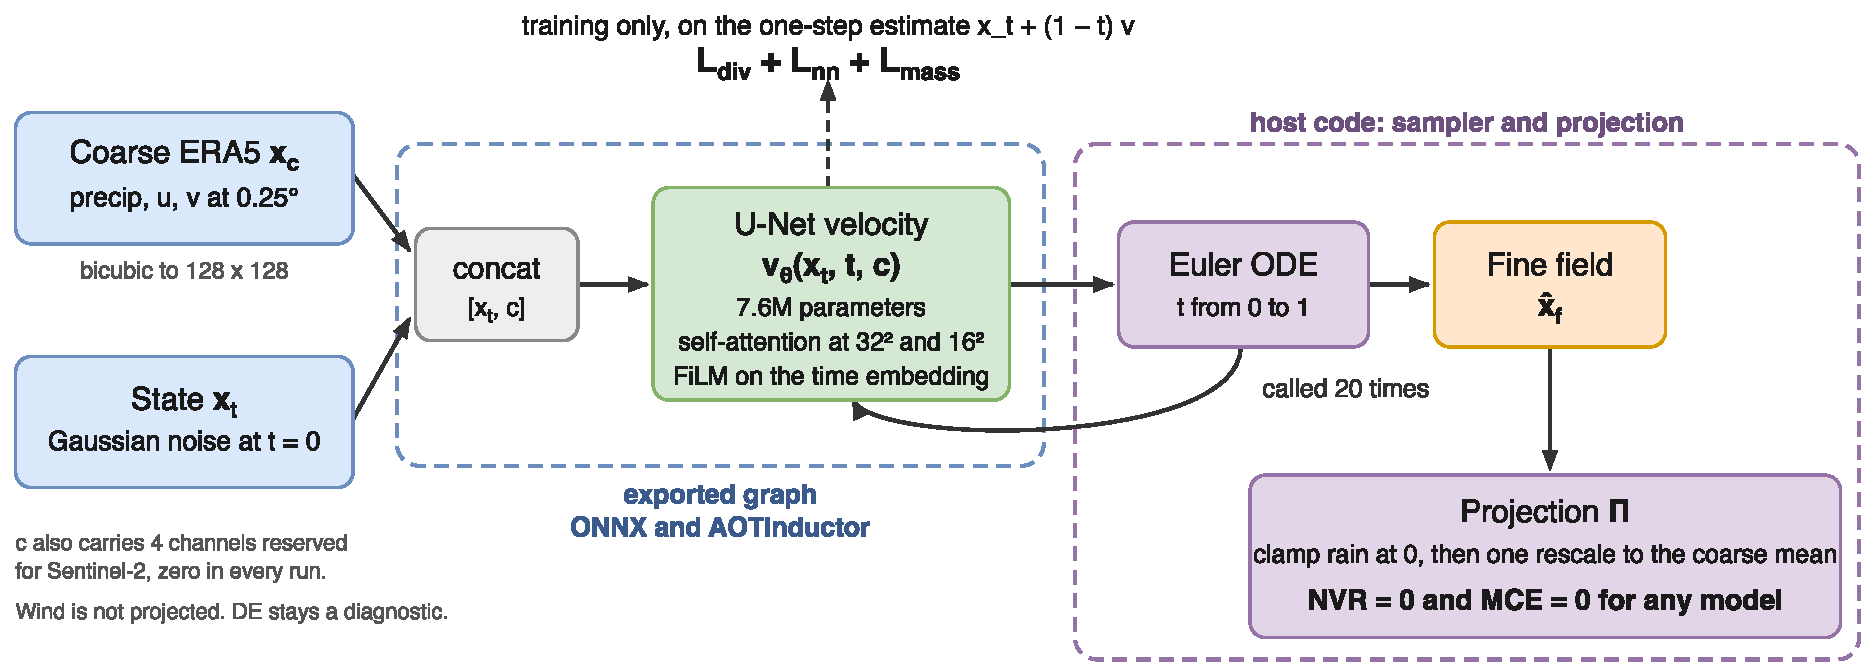
\includegraphics[width=\linewidth]{architecture_corrected_outlined.pdf}
    \figcap{Figure 1.}{This diagram shows PC-RF as trained and served. The 7.6M-parameter U-Net is the
    only exported graph. The Euler sampler and the projection run in host code.}
    \par\vspace{0.20cm}
    \heil{Training} Rectified flow learns a velocity from noise to data, and three
    penalties act on a one-step clean-field estimate. On ERA5, the divergence penalty
    acts on a deformation term (Section 5).
    \begingroup
    \setlength{\abovedisplayskip}{0.10cm}\setlength{\belowdisplayskip}{0.10cm}
    \begin{align}
      \mathcal{L}_{\mathrm{RF}} &= \mathbb{E}\,\bigl\lVert v_\theta(x_t,t,c)-(x_1-x_0)\bigr\rVert_2^2,
      \qquad \hat{x}_1 = x_t+(1-t)\,v_\theta(x_t,t,c)\\
      \mathcal{L} &= \mathcal{L}_{\mathrm{RF}}+\lambda_1\mathcal{L}_{\mathrm{div}}
        +\lambda_2\mathcal{L}_{\mathrm{nn}}+\lambda_3\mathcal{L}_{\mathrm{mass}},
      \qquad \lambda_1=\lambda_2=\lambda_3=1
    \end{align}
    \endgroup
    \heil{Inference} Each of eight ensemble members runs twenty Euler steps. The
    projection then clamps rain at zero and applies one rescale per sample, so the
    domain mean matches the coarse mean $\bar{p}_c$ over land and sea. This domain-level rescaling follows Hess et al.\ (2022), who rescale a trained GAN's precipitation once after training.
    \begingroup
    \setlength{\abovedisplayskip}{0.10cm}\setlength{\belowdisplayskip}{0.10cm}
    \begin{equation}
      \Pi(p) = \max(p,0)\cdot\frac{\bar{p}_c}{\operatorname{mean}\bigl(\max(p,0)\bigr)}
    \end{equation}
    \endgroup
    The rescale needs one positive cell, and the wind is not projected. A divergence-free projection needs a Poisson solve
    over the whole domain, and near-surface convergence is physically real.
  \end{possection}

  \begin{possection}{3.}{Data and Setup}
    \begin{itemize}\setlength{\itemsep}{0.08cm}
      \item The \textbf{coarse input} is ERA5 precipitation and 10\,m $u$, $v$ at
            0.25\textdegree{} over 40--50\textdegree N, 10\textdegree W--5\textdegree E,
            at 00, 06, 12 and 18 UTC.
      \item The \textbf{fine target} is ERA5-Land precipitation at 0.1\textdegree{}
            (about 8 to 11\,km), resampled to $128\times128$, with ocean cells set to
            zero. No fine wind target exists, so the wind target is the upsampled
            coarse wind.
      \item The \textbf{splits} are chronological 80/10/10 on 2020 (1171 training
            samples) and on 2019--2021. The 2020 test set runs from late November to
            31 December.
      \item The \textbf{baselines} are bicubic and our reimplementations of SRCNN,
            SRGAN, DDPM and CorrDiff, scored without the projection.
      \item The \textbf{main run} trained 300 epochs at batch 32 with AdamW (learning
            rate $2\times10^{-4}$) on one A100, about 6.2 GPU-hours.
      \item Each arm was \textbf{one training run} with no fixed seed, and the Sentinel-2 channels were
            zero in every run.
    \end{itemize}
    \par\vspace{0.10cm}
    \begin{takeaway}
      \tklabel{Reference caveat}
      {\color{ncink}\small ERA5-Land precipitation is interpolated from ERA5 forcing
      over a different accumulation window. The perceptual scores therefore measure
      agreement with an interpolant and cannot establish downscaling skill. The
      validity metrics never use the reference.}
    \end{takeaway}
  \end{possection}

  \begin{possection}{4.}{Results}
    \possub{4.1}{Synthetic mechanism check}
    {\centering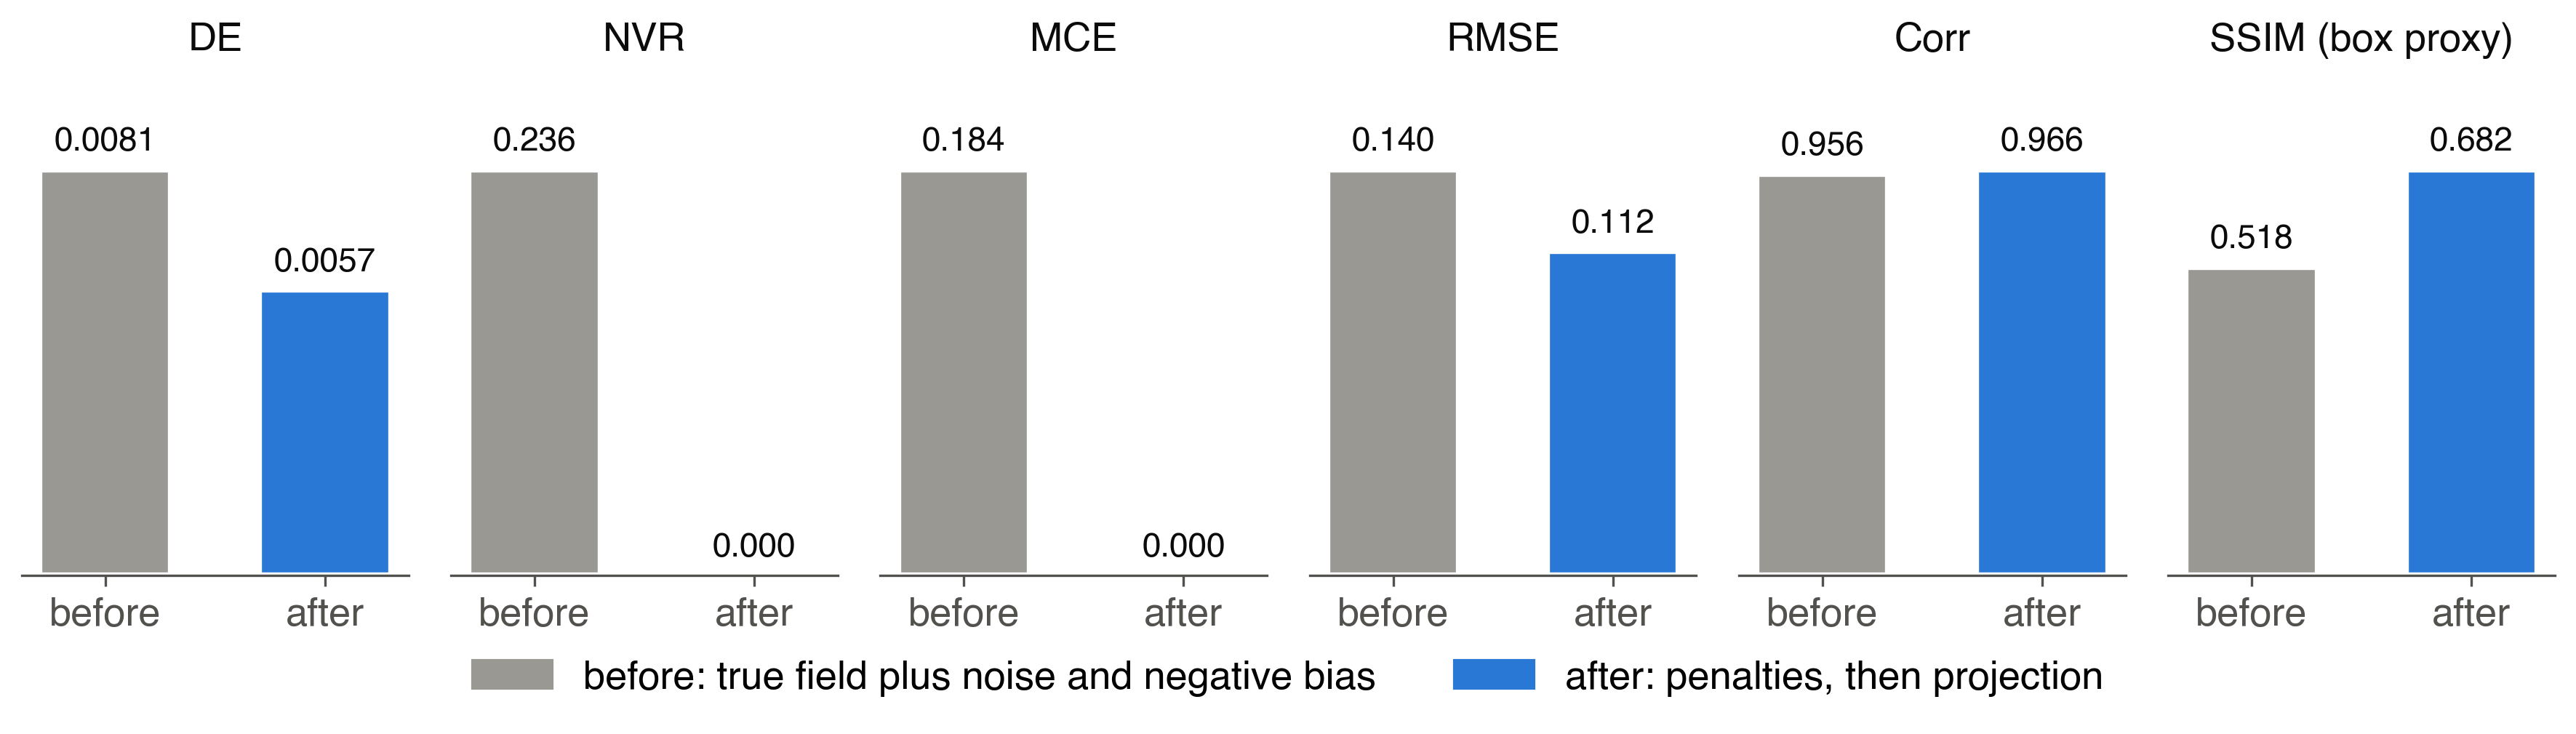
\includegraphics[width=0.88\linewidth]{synthetic_check.png}\par}
    \figcap{Figure 2.}{The check uses one constructed $128\times128$ field with exact
    physics, and no network is trained. The ``before'' field is the truth plus
    correlated noise and a negative bias. The projection drives NVR and MCE to zero,
    and the penalties cut divergence error by about 30\%. The fidelity gain cannot be
    split between the two steps.}
    \par\vspace{0.30cm}

    \possub{4.2}{ERA5 2020: only projected models pass the NVR and MCE checks}
    {\small
    \setlength{\tabcolsep}{9pt}
    \renewcommand{\arraystretch}{1.12}
    \begin{tabularx}{\linewidth}{@{}>{\raggedright\arraybackslash}X rrrrrr@{}}
      \toprule
      \textbf{Model} & \textbf{SSIM}$\uparrow$ & \textbf{PSNR}$\uparrow$ &
      \textbf{CRPS}$\downarrow$ & \textbf{DE} & \textbf{NVR}$\downarrow$ &
      \textbf{MCE}$\downarrow$\\
      \midrule
      Bicubic  & 0.885 & 26.19 & 1.356 & 0.0648 & 0.101 & 0.0003\\
      SRCNN    & 0.833 & 27.74 & 1.461 & 0.0738 & 0.053 & 11.14\\
      SRGAN    & 0.855 & 27.03 & 1.506 & 0.0700 & 0.177 & 13.22\\
      DDPM     & 0.656 & 26.18 & 1.609 & 0.0715 & 0.826 & 7.50\\
      CorrDiff & 0.864 & \textbf{28.38} & \textbf{1.092} & 0.0679 & 0.451 & 6.48\\
      \rowcolor{pcwash}RF-base & 0.912 & 26.39 & 1.188 & 0.0643 & \textbf{0} & \textbf{0}\\
      \rowcolor{pcwash}PC-RF   & \textbf{0.914} & 26.59 & 1.149 & 0.0644 & \textbf{0} & \textbf{0}\\
      \bottomrule
    \end{tabularx}}
    \figcap{Table 1.}{Shaded rows carry the projection. RF-base trained 200 epochs at
    batch 16, and the other learned models trained 300. For the four sampled models,
    CRPS uses the 8 members and the other metrics use their mean, while bicubic, SRCNN
    and SRGAN give one output, so the two groups are not strictly comparable. SSIM, PSNR
    and CRPS also average two wind channels whose target is the upsampled coarse wind.
    MCE is a relative error of the domain mean, not a water amount, and DE is the ERA5
    deformation term, a diagnostic in standardized grid units.}
    \par\vspace{0.30cm}

  \end{possection}

  \vspace{-0.40cm}
\end{column}

%% ==================== COLUMN 2 ====================
\begin{column}{0.485\textwidth}

  \begin{possection}{4.}{Results (continued)}
    \possub{4.3}{One year at a matched budget}
    {\small
    \setlength{\tabcolsep}{9pt}
    \renewcommand{\arraystretch}{1.10}
    \begin{tabularx}{\linewidth}{@{}>{\raggedright\arraybackslash}X rrrr@{}}
      \toprule
      \textbf{Arm (200 epochs, batch 16)} & \textbf{SSIM}$\uparrow$ & \textbf{PSNR}$\uparrow$ &
      \textbf{CRPS}$\downarrow$ & \textbf{DE}\\
      \midrule
      Full PC-RF                & 0.912 & 26.54 & 1.161 & 0.0634\\
      No divergence penalty     & 0.912 & \textbf{26.58} & \textbf{1.146} & 0.0649\\
      No non-negativity penalty & 0.913 & 26.55 & 1.160 & 0.0644\\
      No mass penalty           & \textbf{0.915} & 26.50 & 1.166 & 0.0639\\
      RF-base (no penalties)    & 0.913 & 26.40 & 1.186 & 0.0643\\
      \bottomrule
    \end{tabularx}}
    \figcap{Table 2.}{The penalty arms tie RF-base on SSIM and lead it slightly on PSNR
    and CRPS. With one seed per arm, that lead cannot be separated from run-to-run
    variation. DE is the same ERA5 deformation term. The same RF-base checkpoint gives
    the Table 1 row, scored there with a fresh 8-member sample.}
    \par\vspace{0.30cm}

    \possub{4.4}{Three years at a matched budget: a tie}
    \begin{center}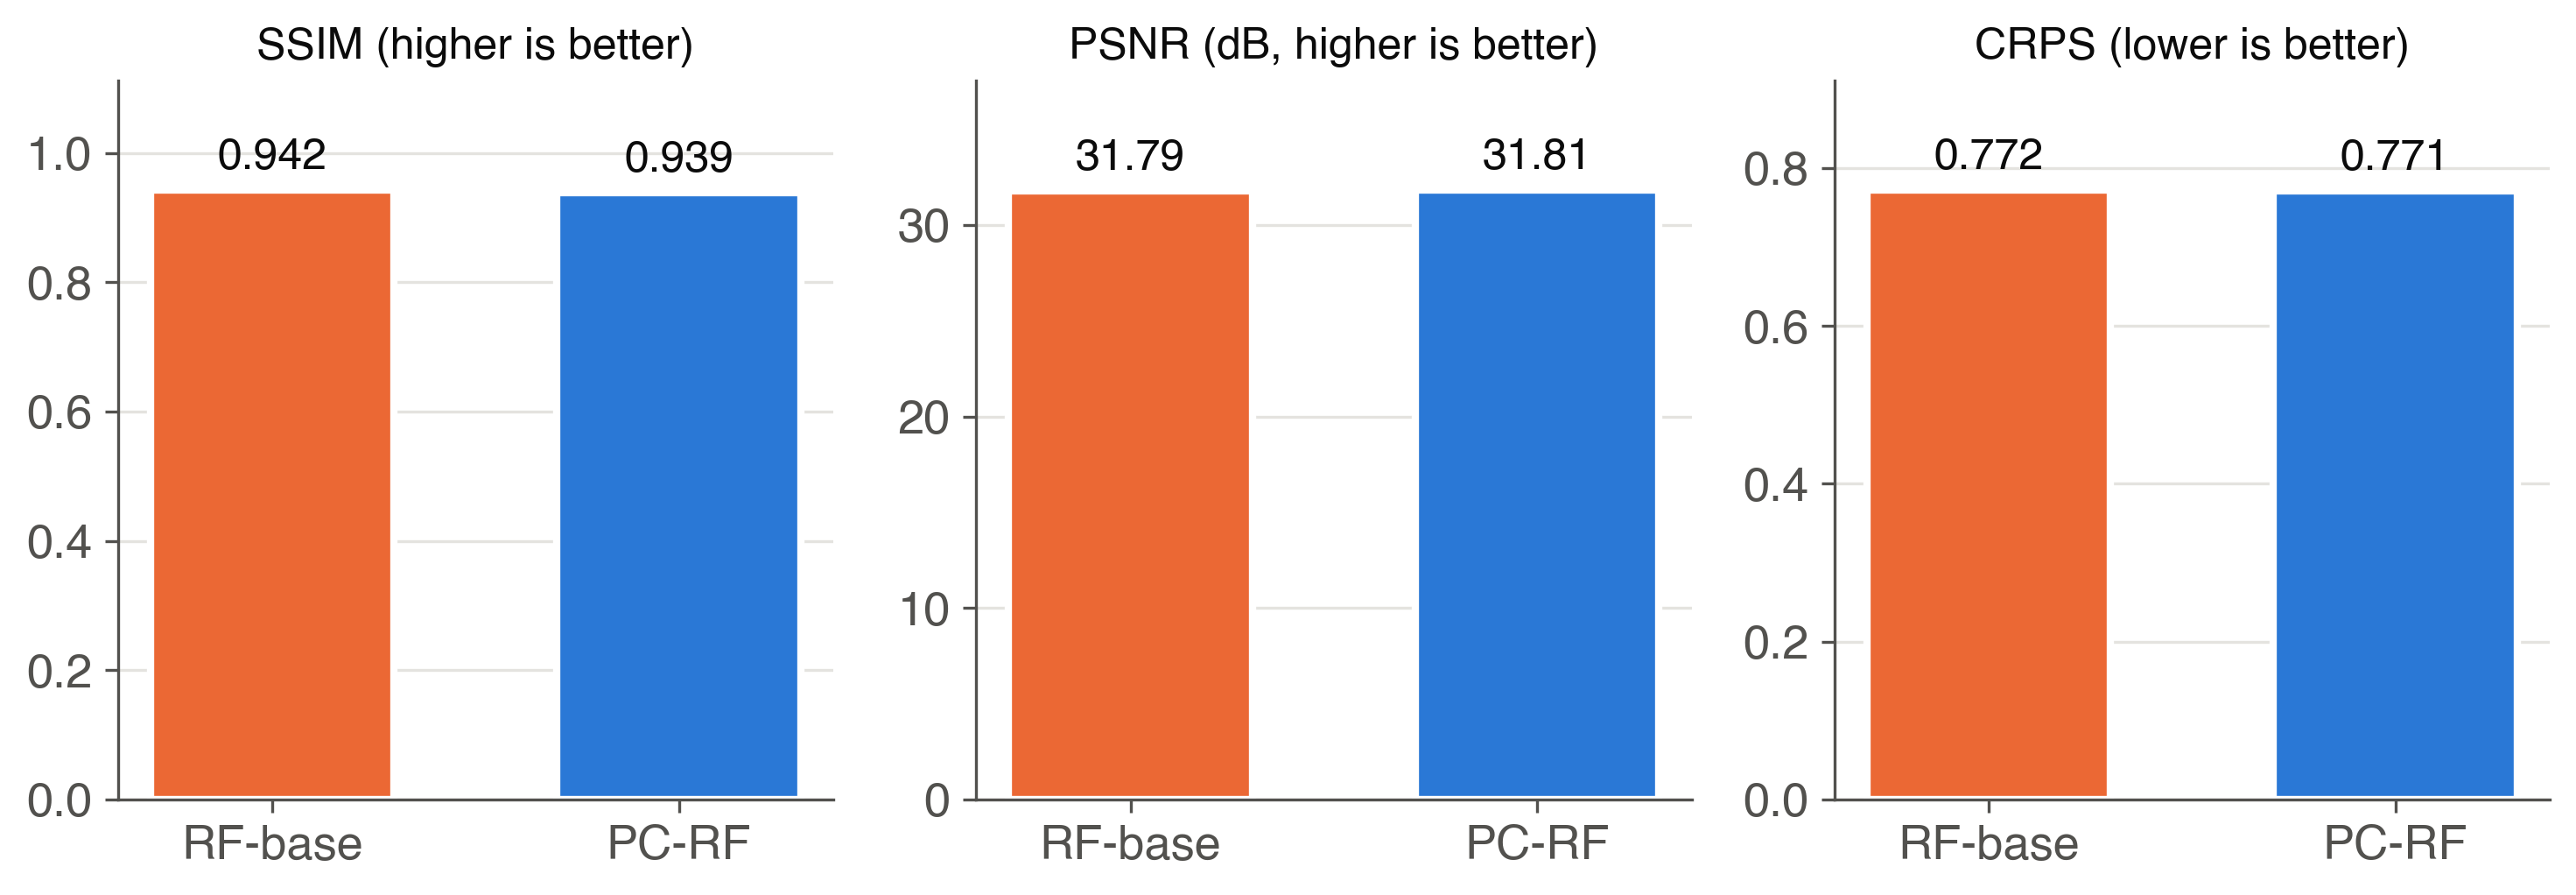
\includegraphics[width=0.80\linewidth]{threeyr_null.png}\end{center}
    \figcap{Figure 3.}{Every arm trained 100 epochs on 2019--2021. RF-base matches
    PC-RF on every perceptual score, and both keep NVR and MCE at zero up to rounding.
    These scores mix rain and wind.}
    \par\vspace{0.18cm}
    \begin{takeaway}
      \tklabel{Result}
      {\color{ncink}\normalsize The penalties add no measurable perceptual gain at a
      matched three-year budget. The validity guarantee comes from the projection.}
    \end{takeaway}
  \end{possection}

  \vspace{-0.20cm}
  \begin{possection}{5.}{What the Checks Certify}
    \begin{itemize}\setlength{\itemsep}{0.02cm}
      \item \textbf{Reference-free}: NVR (negative-value rate) and MCE (mass-conservation
            error) need only the generated field and its coarse input.
      \item \textbf{Certificates}: after the projection both are zero for any model, up
            to float32 rounding, so they report the inference step and cannot rank two
            projected models.
      \item \textbf{Diagnostic}: On ERA5, a latitude sign error makes DE (divergence
            error) measure a deformation term, not divergence, and it carries no guarantee. The
            reference wind is upsampled coarse wind, whose own DE is 0.0648 on
            2020 and 0.0567 on 2019--2021.
      \item \textbf{Necessary, not sufficient}: a field can pass every check and still
            be wrong.
    \end{itemize}
    \par\vspace{0.12cm}
    \noindent
    \begin{minipage}[t]{0.52\linewidth}
      \vspace{0pt}
      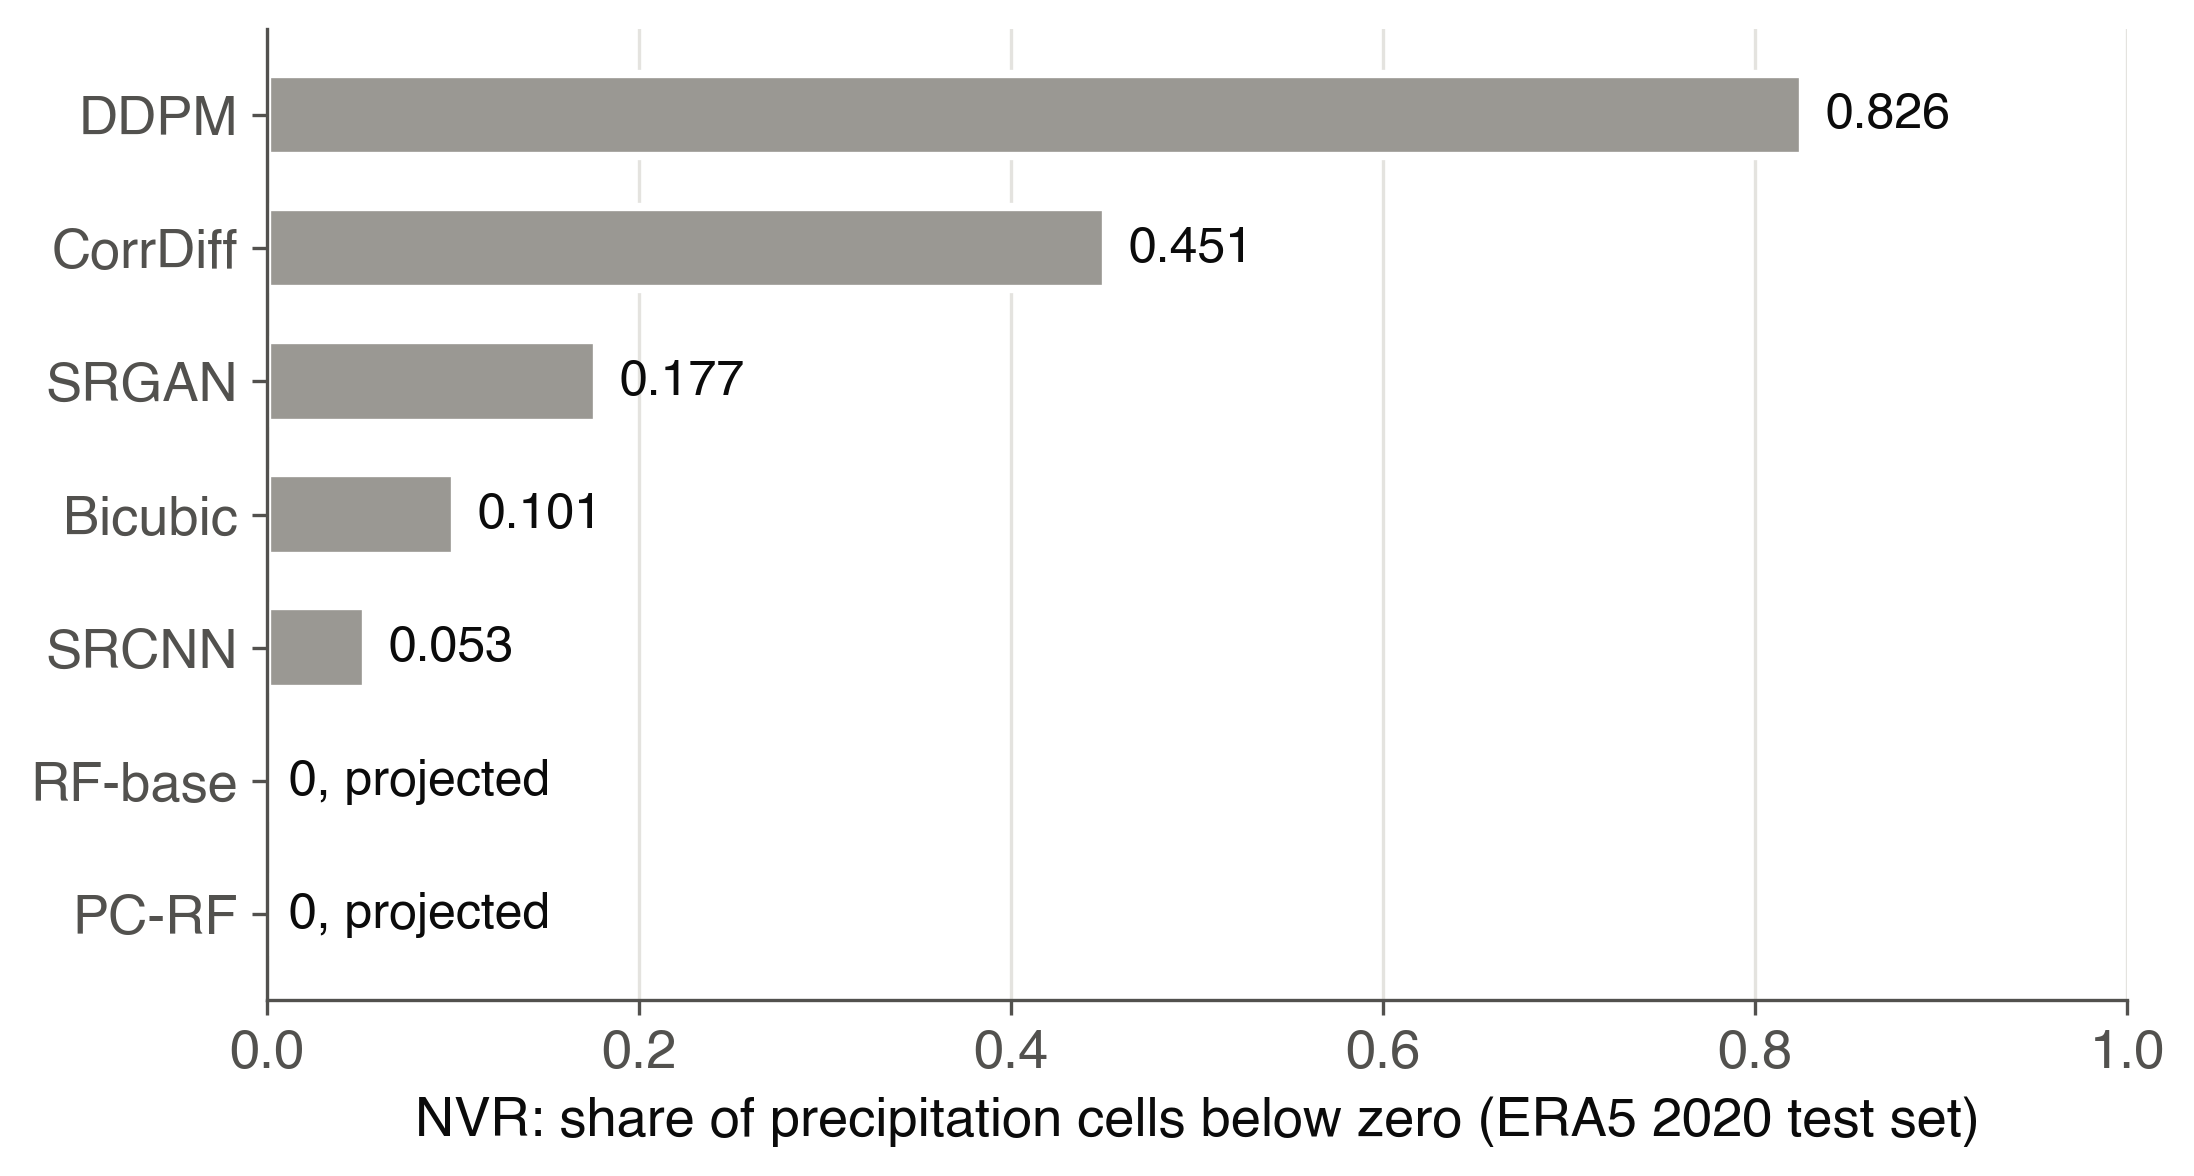
\includegraphics[width=\linewidth]{nvr_2020.png}
    \end{minipage}\hfill
    \begin{minipage}[t]{0.45\linewidth}
      \vspace{0pt}\raggedright
      {\color{ncmuted}\normalsize\textbf{Figure 4.}\hspace{0.3em}The bars show the share of
      precipitation cells below zero on the ERA5 2020 test set. Every model scored without
      the projection fails the gate, bicubic included. Bicubic's negatives come from
      interpolation ringing, and a clamp would remove them.\par}
    \end{minipage}
    \par\vspace{0.14cm}
    \begin{takeaway}
      \tklabel{Recommendation}
      {\color{ncink}\normalsize Run NVR and MCE first, and keep DE beside them as a diagnostic.}
    \end{takeaway}
  \end{possection}

  \vspace{-0.20cm}
  \begin{possection}{6.}{From PyTorch to Production}
    \heil{Export the network, not the sampler} The exported graph is one velocity
    call, $v_\theta(x_t,t,c)$. The Euler loop and the projection stay in host code,
    mirrored in Python and Rust.
    \par\vspace{0.12cm}
    \heil{Serving on one A100} One request (20 steps plus the projection, batch 1)
    takes 91.7\,ms in eager PyTorch, 43.3\,ms with AOTInductor, 49.1\,ms with
    \apicode{torch.compile}, and 65.5\,ms with ONNX Runtime, which copies through the
    host every step. The weights are random in the trained architecture.
    \par\vspace{0.06cm}
    \begin{center}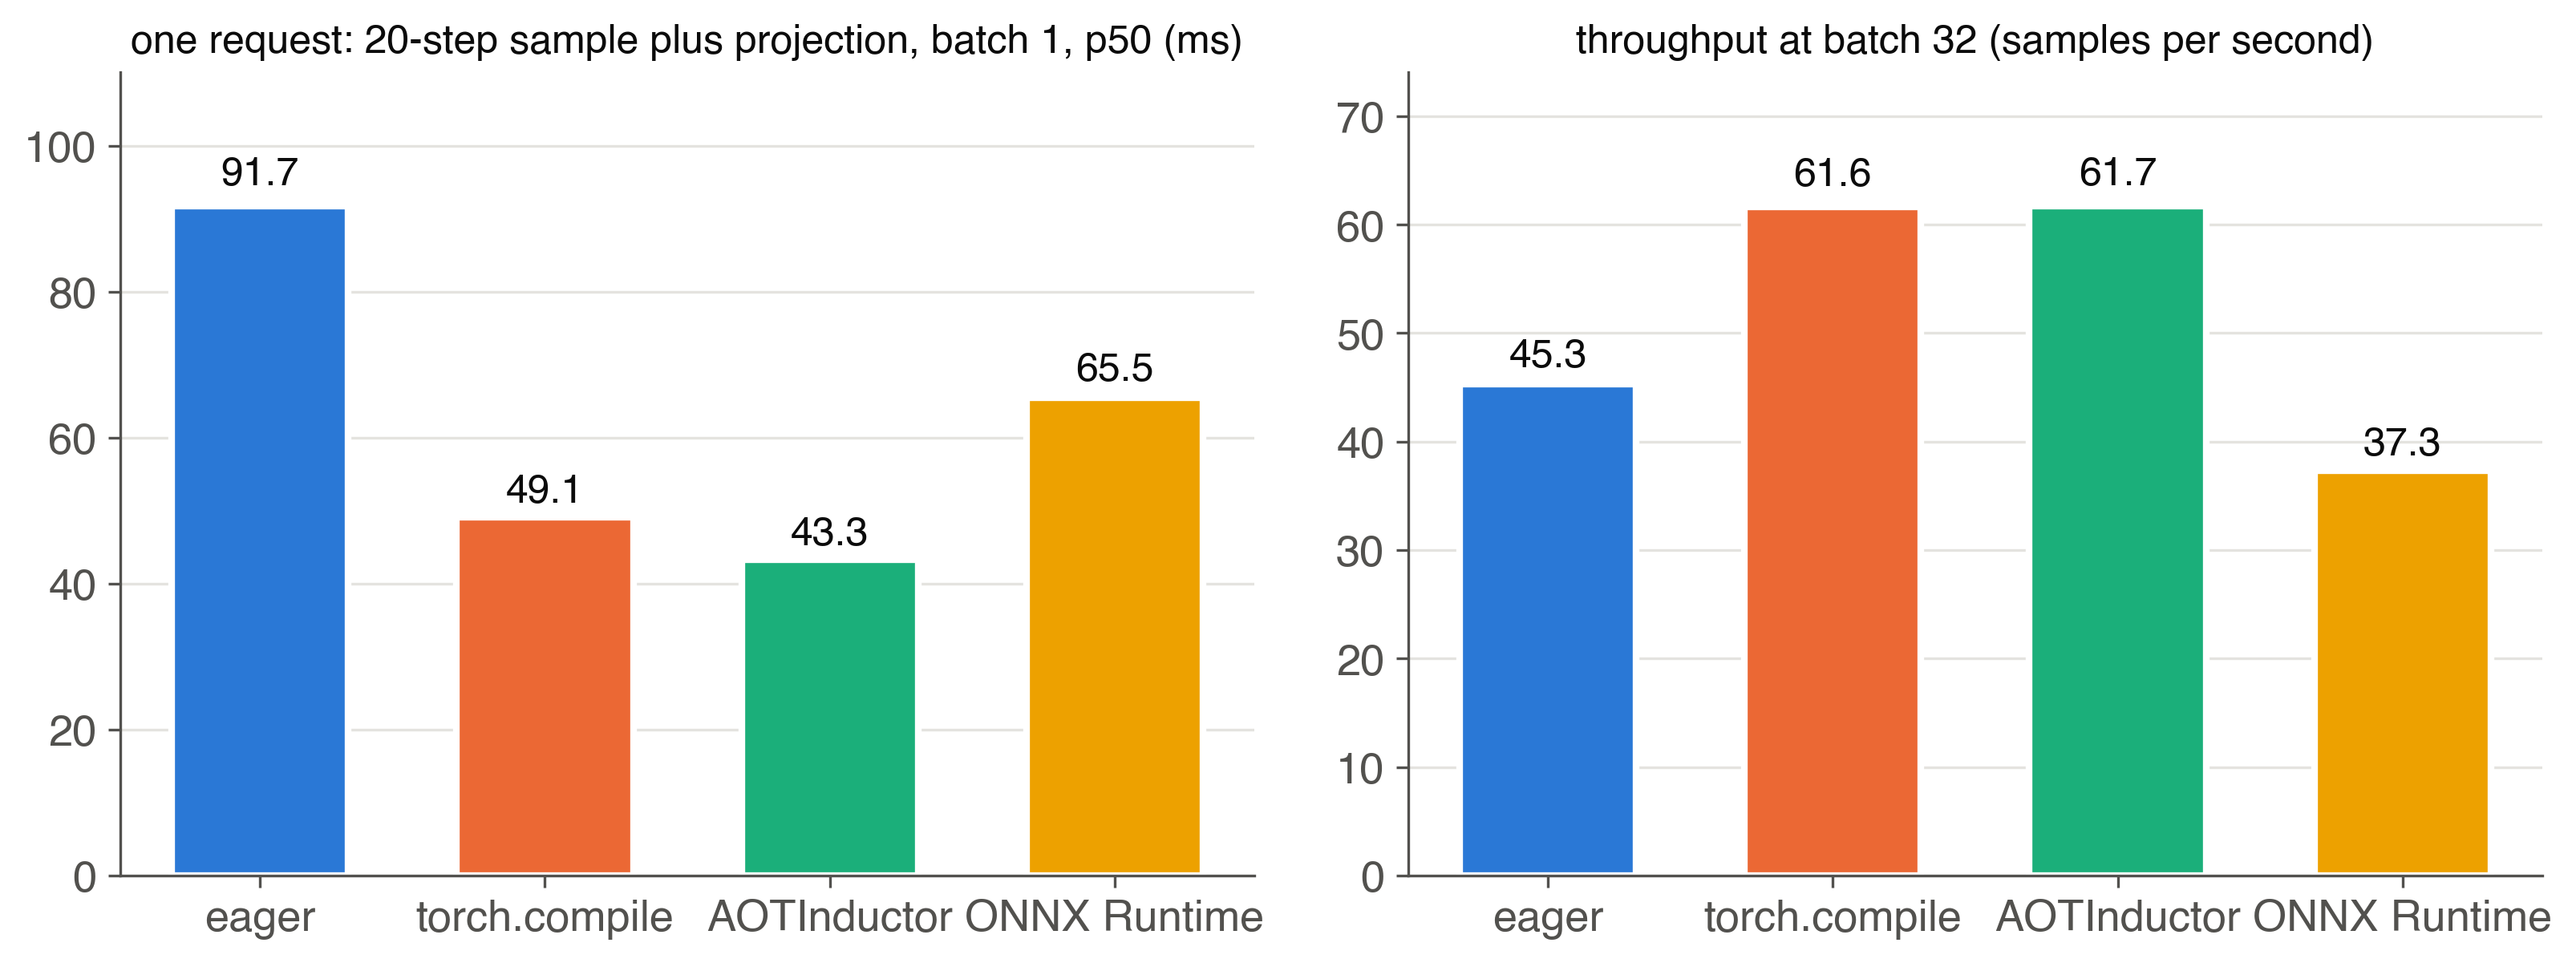
\includegraphics[width=0.72\linewidth]{serving_bench.png}\end{center}
    \figcap{Figure 5.}{The panels show one request and throughput at batch 32 on an
    A100-SXM4-40GB, with random weights. With TF32 off, \apicode{torch.compile} and
    AOTInductor match eager within a maximum absolute difference of
    $2\times10^{-6}$, and NVR stays at zero on every backend. The Rust service and Ray
    Serve were tested on a demo-scale export, and every model here trained on one GPU.}
  \end{possection}

  \vspace{-0.20cm}
  \begin{possection}{7.}{Conclusion and Future Work}
    \begin{itemize}\setlength{\itemsep}{0.02cm}
      \item The projection carries the validity guarantee, and the penalties add no
            measurable perceptual gain at a matched three-year budget.
      \item The ERA5-Land reference is interpolated, so it cannot show downscaling skill.
      \item The projection matches the land-and-sea coarse mean, which the reference does not match.
      \item We used one domain and one run per arm, tested in autumn and early winter, with no extremes test.
      \item Baselines were scored without the projection, which any of them could apply.
      \item On ERA5, a sign error makes the divergence penalty and DE measure deformation.
      \item An independent target with its own precipitation would test the mass penalty.
    \end{itemize}
  \end{possection}

  \vspace{-0.40cm}
\end{column}

\end{columns}
\vfill
\begin{possection}{8.}{Resources}
  \noindent
  \qrcell{Repo}{https://github.com/arunshar/pcrf-aias2026-talk}{github.com/arunshar/pcrf-aias2026-talk}\hfill
  \qrcell{Slides}{https://github.com/arunshar/pcrf-aias2026-talk/blob/main/slides/PCRF_AIAS2026_slides.pdf}{pcrf-aias2026-talk/slides/PCRF\_AIAS2026\_slides.pdf}\hfill
  \qrcell{Video}{https://youtu.be/xyiUB-ehX8g}{youtu.be/xyiUB-ehX8g}\hfill
  \qrcell{Paper}{https://github.com/arunshar/pcrf-aias2026-talk/blob/main/paper/PCRF_AIAS2026_paper.pdf}{pcrf-aias2026-talk/paper/PCRF\_AIAS2026\_paper.pdf}
\end{possection}

\end{frame}
\end{document}
